\section{Damping--Solver Stability and Loss-Landscape Analysis}
\label{sec:track-d}

Numerical stiffness -- a system whose fastest and slowest timescales differ by
orders of magnitude -- is where explicit integrators are classically expected
to struggle. This study sweeps the pendulum's damping coefficient
$\mu\in\{0.1,0.5,1.0,2.0,5.0,8.0\}$ (Equation~\ref{eq:pendulum}; the
dimensionless damping ratio is $\zeta=\mu/(2\sqrt{g/L})$, from $0.016$ to
$1.28$) against four explicit Runge-Kutta solvers (Euler, Midpoint, RK4,
Tsit5), to map which $(\text{solver},\mu)$ combinations train and which do
not, and to test whether any failure is a stiffness effect. Every cell uses
the adopted pendulum recipe (Table~\ref{tab:train-settings}: $[2,10,2]$,
$G=8$, 360 parameters, training window $[0,5]$ of $[0,10]$), data spacing
$\Delta t=0.05$ with two substeps, so the integration step is $h=0.025$, and
2{,}000 epochs.

As the analysis below shows, this sweep never reaches a stiff regime: the
largest ratio between the system's two timescales is $4.3$, at $\mu=8$. It
is therefore a study of how \emph{damping} interacts with the solver and with
training, not of stiffness in the numerical-analysis sense. A genuinely stiff
test would need a system with a timescale ratio of $10^3$ or more.

\begin{expectbox}
\expectrow{Question}{Does stronger damping push some (solver, $\mu$) combinations outside the solver's stability region, so that lower-order explicit solvers fail?}
\expectrow{Expected}{If any cell leaves its solver's stability region, that cell should diverge, and lower-order solvers should fail first.}
\expectrow{Observed}{Linear stability theory predicts no divergence anywhere, for the true system and for the trained networks, and none occurs. Every observed failure traces to the random seed, not to the solver.}
\end{expectbox}

\subsection{The stability question resolves quickly}

Linearizing the true system at its equilibrium gives eigenvalues
$\lambda = \big({-\mu\pm\sqrt{\mu^2-4g/L}}\big)/2$. For every underdamped
$\mu<2\sqrt{g/L}\approx6.26$, $|\lambda|=\sqrt{g/L}\approx3.13$ is constant, so
$h|\lambda|\approx0.078$ at $h=0.025$, far inside even Euler's stability
interval $h|\lambda|\le2$ on the negative real axis
(Equation~\ref{eq:stability-function}, \cite{hairer1996solving}). The
overdamped case $\mu=8$ has real eigenvalues $-1.51$ and $-6.49$, a
timescale ratio of only $4.3$, and $h|\lambda_{\text{fast}}|\approx0.162$,
still comfortably stable.

What the integrator actually steps, however, is the \emph{learned} field,
not the true one. Its Jacobian was evaluated along the true trajectory for
all 24 seed-42 models, every solver at every $\mu$. The largest eigenvalue
magnitude per model is $3.5$--$11.8$, up to about four times the true
system's, which is consistent with the Lipschitz estimates of
Section~\ref{sec:phase2}. Even so, $h|\lambda|\le0.30$ for every model, still
well inside every solver's stability region. This predicts, and the sweep confirms, zero
divergences: across all 24 cells not one run produced a non-finite gradient
at any point in training. All four solvers are explicit Runge-Kutta methods
with a bounded stability region, and no implicit solver is implemented in
this project, so this analysis cannot say how an implicit method would
behave on a genuinely stiff system.

\subsection{What actually drives the failures: initialization}

Each cell is classified from its training record alone. A run is
\emph{diverged} if it was aborted by the non-finite guard
(Algorithm~\ref{alg:train}); it is \emph{converged} if it had no non-finite
steps, its best training MSE is below $10^{-2}$, and its final training MSE
is no more than $10\times$ its best; every other run is \emph{not
converged}. No run in this study diverged, so every failure below is a run
that stayed finite but never fit, or fit and then regressed. The $10^{-2}$
threshold is coarse: $\mu=0.5$ cells at $4.6$--$9.2\times10^{-3}$ count as
converged while $\mu=0.1$ cells at $1.7$--$3.0\times10^{-2}$ do not, so
verdicts near the threshold should be read together with the MSE values in
Table~\ref{tab:stiffness-single-seed}.

\begin{table}[!ht]
\centering
\footnotesize
\renewcommand{\arraystretch}{1.15}
\caption{Original 24-cell sweep (single seed 42): best training MSE and
verdict. ``Not conv.'' is not converged under the rule above; no cell
diverged.}
\label{tab:stiffness-single-seed}
\begin{tabularx}{\textwidth}{@{}C{1.3cm} X X X X@{}}
\toprule
\hdrrow \thh{Damping coefficient $\mu$} & \thh{Euler} & \thh{Midpoint} & \thh{RK4} & \thh{Tsit5}\\
\midrule
0.1 & not conv., $1.7\times10^{-2}$ & not conv., $3.0\times10^{-2}$ & not conv., $2.2\times10^{-2}$ & not conv., $2.4\times10^{-2}$\\
0.5 & \textbf{converged}, $4.6\times10^{-3}$ & \textbf{converged}, $7.9\times10^{-3}$ & \textbf{converged}, $4.7\times10^{-3}$ & \textbf{converged}, $9.2\times10^{-3}$\\
1.0 & not conv., $1.0\times10^{-1}$ & converged, $5.4\times10^{-4}$ & converged, $5.3\times10^{-4}$ & converged, $4.0\times10^{-4}$\\
2.0 & not conv., $1.8\times10^{-2}$ & not conv., $1.8\times10^{-2}$ & not conv., $1.8\times10^{-2}$ & not conv., $1.8\times10^{-2}$\\
5.0 & converged, $6.1\times10^{-5}$ & converged, $7.0\times10^{-5}$ & converged, $6.9\times10^{-5}$ & converged, $6.8\times10^{-5}$\\
8.0 & converged, $2.1\times10^{-5}$ & converged, $2.3\times10^{-5}$ & converged, $2.6\times10^{-5}$ & converged, $2.6\times10^{-5}$\\
\bottomrule
\end{tabularx}
\end{table}

\begin{figure}[htbp]
\centering
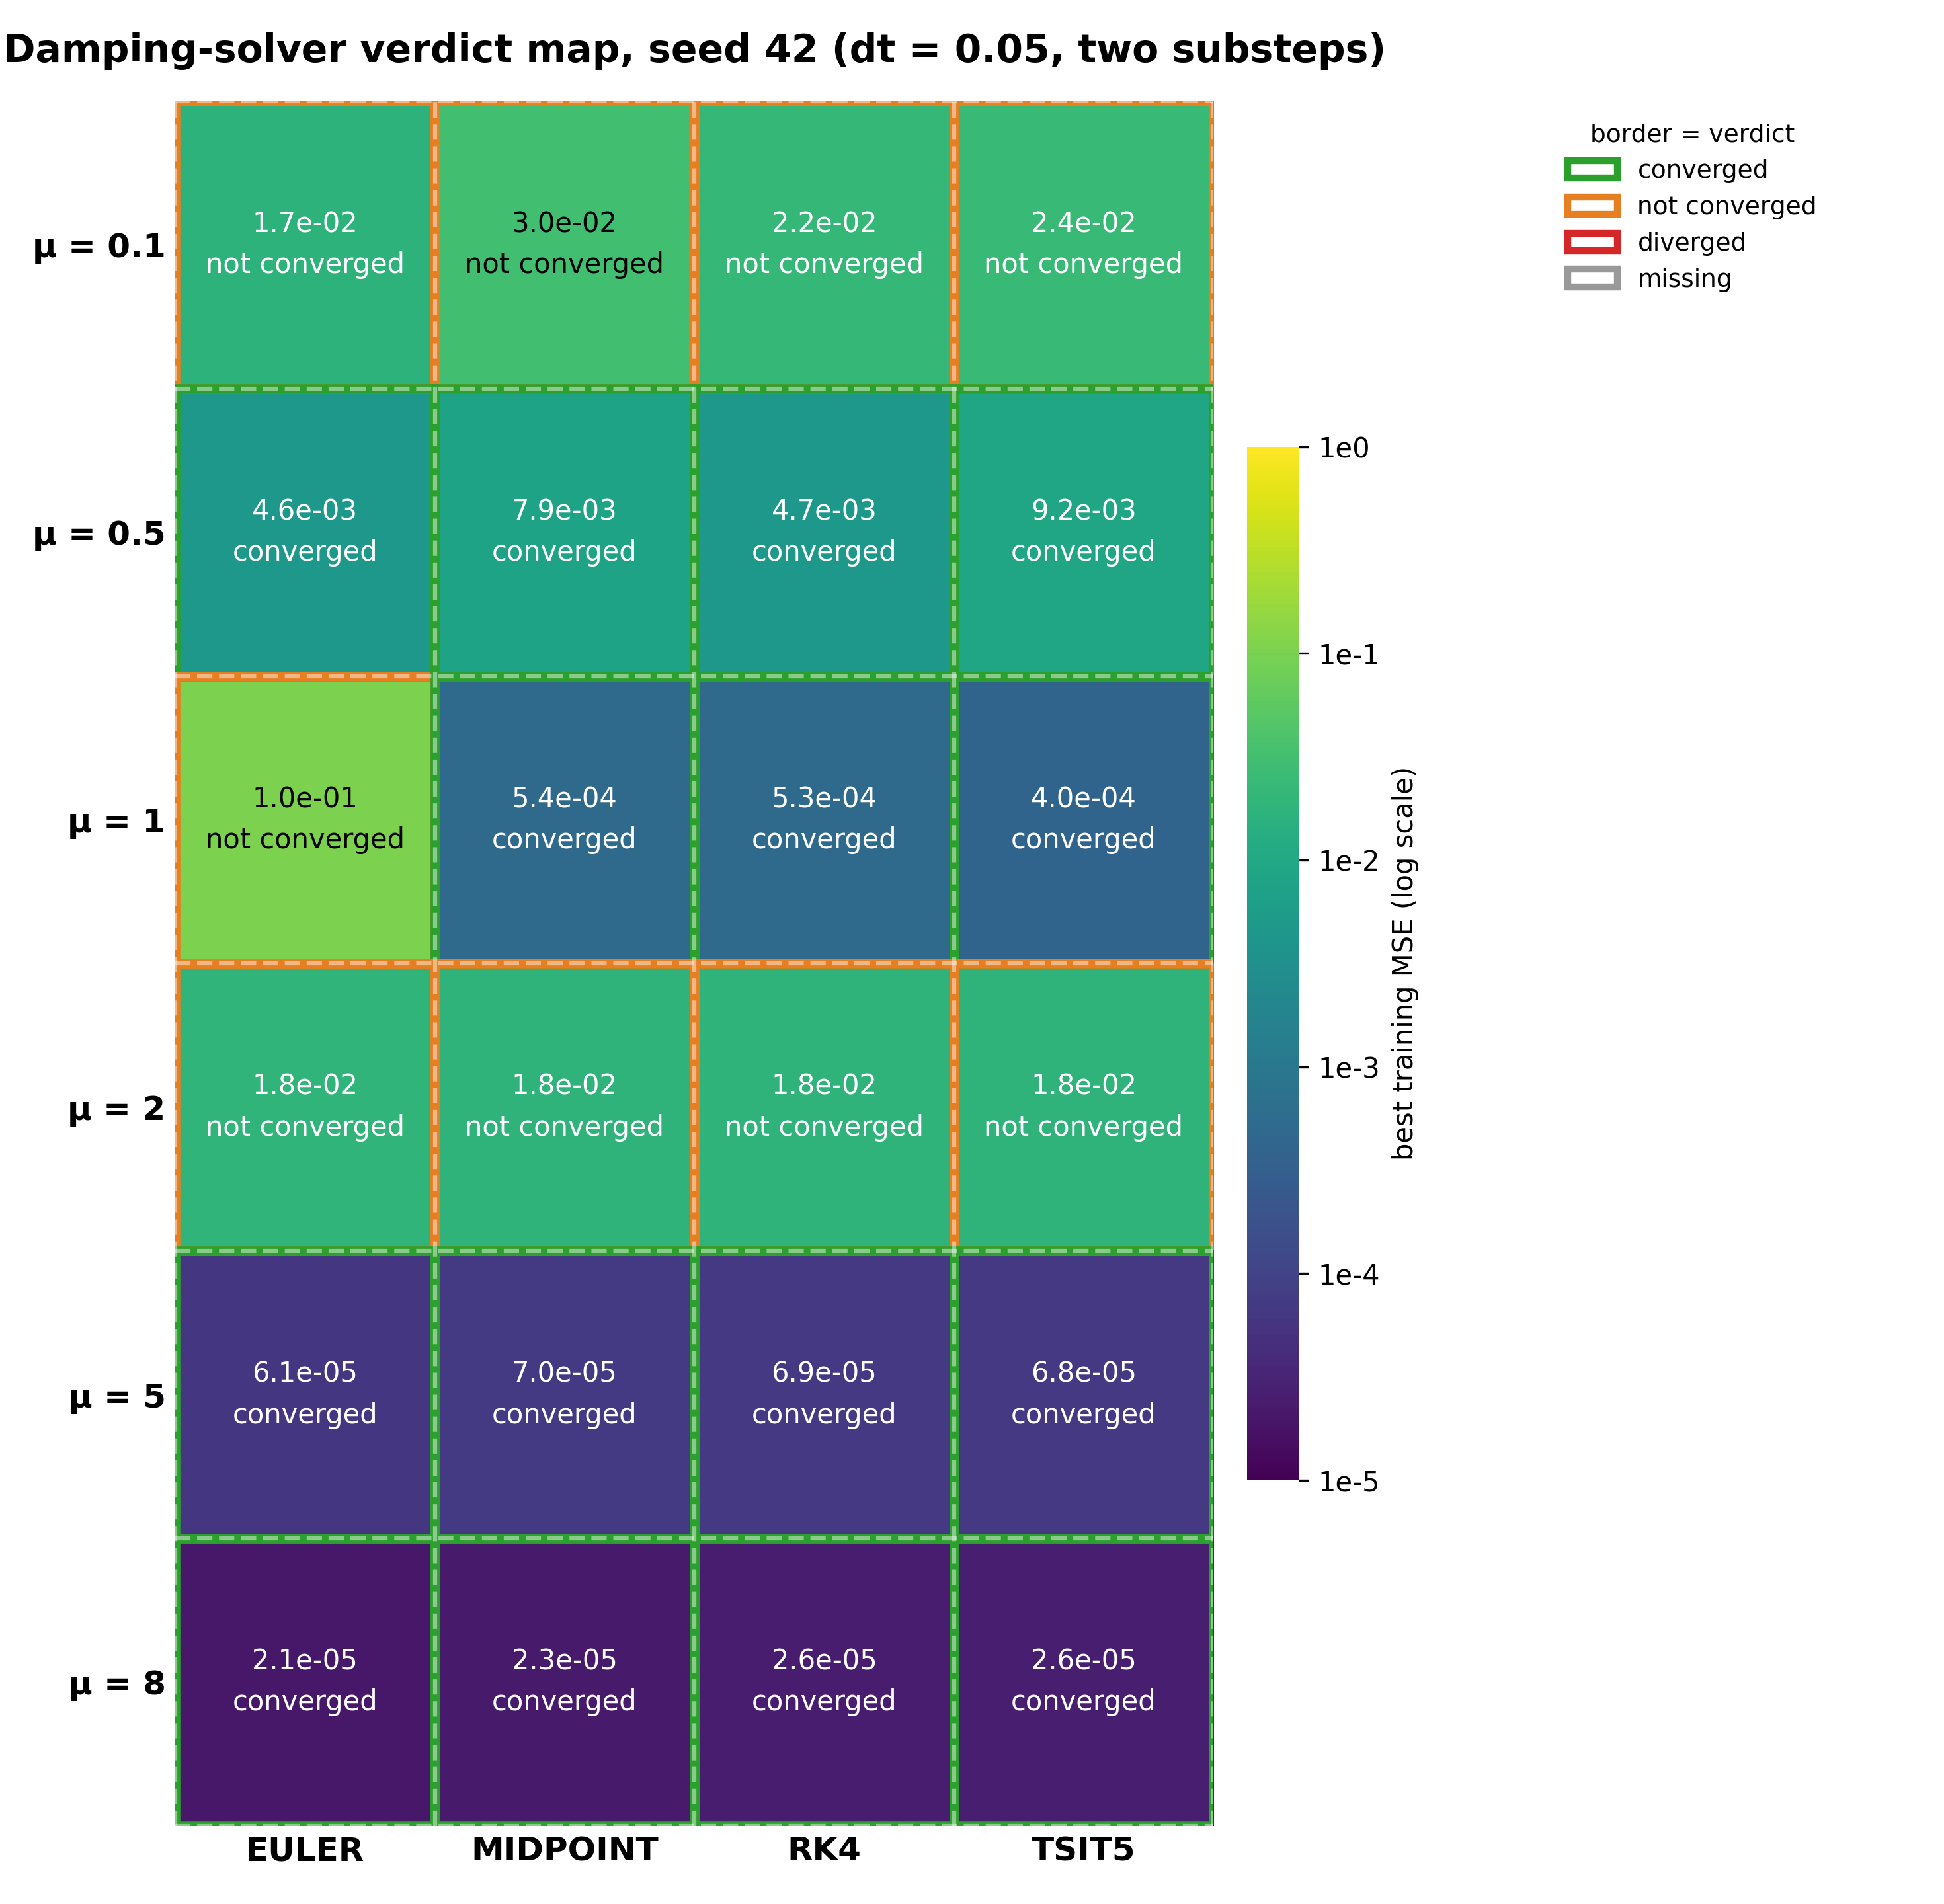
\includegraphics[width=0.7\linewidth]{figures/track_d/stability_heatmap_dt0.05.png}
\caption{Verdict map of the 24-cell single-seed sweep ($\Delta t=0.05$, two
substeps). Each cell shows its best training MSE and verdict under the rule
above; the border color repeats the verdict.}
\label{fig:stability-heatmap}
\end{figure}

Two anomalies stand out in Table~\ref{tab:stiffness-single-seed} and
Figure~\ref{fig:stability-heatmap}: $\mu=2.0$ fails identically across all
four solvers to two significant figures, and $\mu=1.0$ fails only for Euler.
Retraining Euler at $\mu=2.0$ with two more seeds isolates the cause (seed 42:
not converged, $1.82\times10^{-2}$; seed 1: not converged,
$1.68\times10^{-2}$; seed 7:
\textbf{converged}, $7.09\times10^{-5}$) -- the trap depends on the random
initialization. Extending this to all four solvers $\times$ six $\mu$
$\times$ three seeds (72 cells, checkpoints saved throughout) confirms the
pattern generally: only the two extremes ($\mu=0.1$, uniformly hard;
$\mu\in\{5.0,8.0\}$, uniformly easy) hold their verdict across every seed.
Every transitional $\mu\in\{0.5,1.0,2.0\}$ has at least one of three seeds
land in a bad local minimum, and at $\mu=1.0$ two \emph{different} seeds fail
for two different reasons: seed 1 produces a universally bad initialization
shared by all four solvers (MSE $\approx9.7\text{--}9.8\times10^{-2}$, the
same signature as the $\mu=2.0$ shared trap), while seed 42 carries a second,
Euler-specific failure on top of it. Euler's apparent $\mu=1.0$ weakness in
Table~\ref{tab:stiffness-single-seed} is therefore the sum of two separate
effects, one shared and one solver-specific, compressed into a single
misleading number.

\begin{keypoint}[Consequence for the original heatmap]
The 24-cell sweep used one shared seed for all four solvers. All four solvers
failing identically at $\mu=2.0$ reflects four solvers inheriting the same
coin flip from a shared initialization, at this step size the seed$\times\mu$
interaction determines outcome far more than solver choice does.
\end{keypoint}

\subsection{The mechanism: a genuine spurious equilibrium}

For the trapped $\mu=2.0$ models, the learned field is far from zero at the
true equilibrium: $|f_\theta(0,0)|\in[2.65,2.88]$ across all four solvers'
own trained models. A coarse grid search first located a nearby point where
$|f_\theta|=0.0086$. To confirm that this is a genuine equilibrium, Newton's
method was run on $f_\theta(\mathbf u)=\mathbf 0$ from that point, for each
solver's model (Table~\ref{tab:spurious-eq}). All four converge to a true
zero of the learned field, to a residual of $\sim10^{-6}$, at almost the same
location, about $0.05$ from the true equilibrium. At that point the
Jacobian's eigenvalues are a complex pair with negative real part, so the
point is a \emph{stable spiral}: trajectories near it wind inward and stop
there. Four networks trained from the same initial weights but through four
different integrators learned essentially the same wrong but genuine,
attracting fixed point (Figure~\ref{fig:phase-portraits}).

\begin{table}[!ht]
\centering
\footnotesize
\renewcommand{\arraystretch}{1.12}
\caption{Equilibria of the learned field for the trapped $\mu=2.0$ models
(seed 42), found by Newton's method on $\mathbf f_\theta(\mathbf u)=\mathbf 0$.
The true equilibrium is $(0,0)$, where the true Jacobian has eigenvalues
$-1\pm2.97i$.}
\label{tab:spurious-eq}
\begin{tabular}{@{}L{2.0cm} C{2.2cm} C{3.2cm} C{2.0cm} C{3.2cm}@{}}
\toprule
\hdrrow \thh{Solver} & \thh{$|\mathbf f_\theta(0,0)|$} & \thh{Learned equilibrium $(\theta,\omega)$} & \thh{Residual $|\mathbf f_\theta|$} & \thh{Jacobian eigenvalues there}\\
\midrule
Euler & 2.77 & $(-0.049,\,+0.016)$ & $1.5\times10^{-6}$ & $-0.62\pm3.35i$\\
Midpoint & 2.88 & $(-0.049,\,+0.014)$ & $1.2\times10^{-6}$ & $-0.45\pm3.94i$\\
RK4 & 2.65 & $(-0.047,\,+0.014)$ & $6.7\times10^{-7}$ & $-0.48\pm3.96i$\\
Tsit5 & 2.86 & $(-0.050,\,+0.016)$ & $1.5\times10^{-6}$ & $-0.47\pm3.93i$\\
\bottomrule
\end{tabular}
\end{table}

\begin{figure}[htbp]
\centering
\begin{minipage}[t]{0.48\textwidth}
\centering
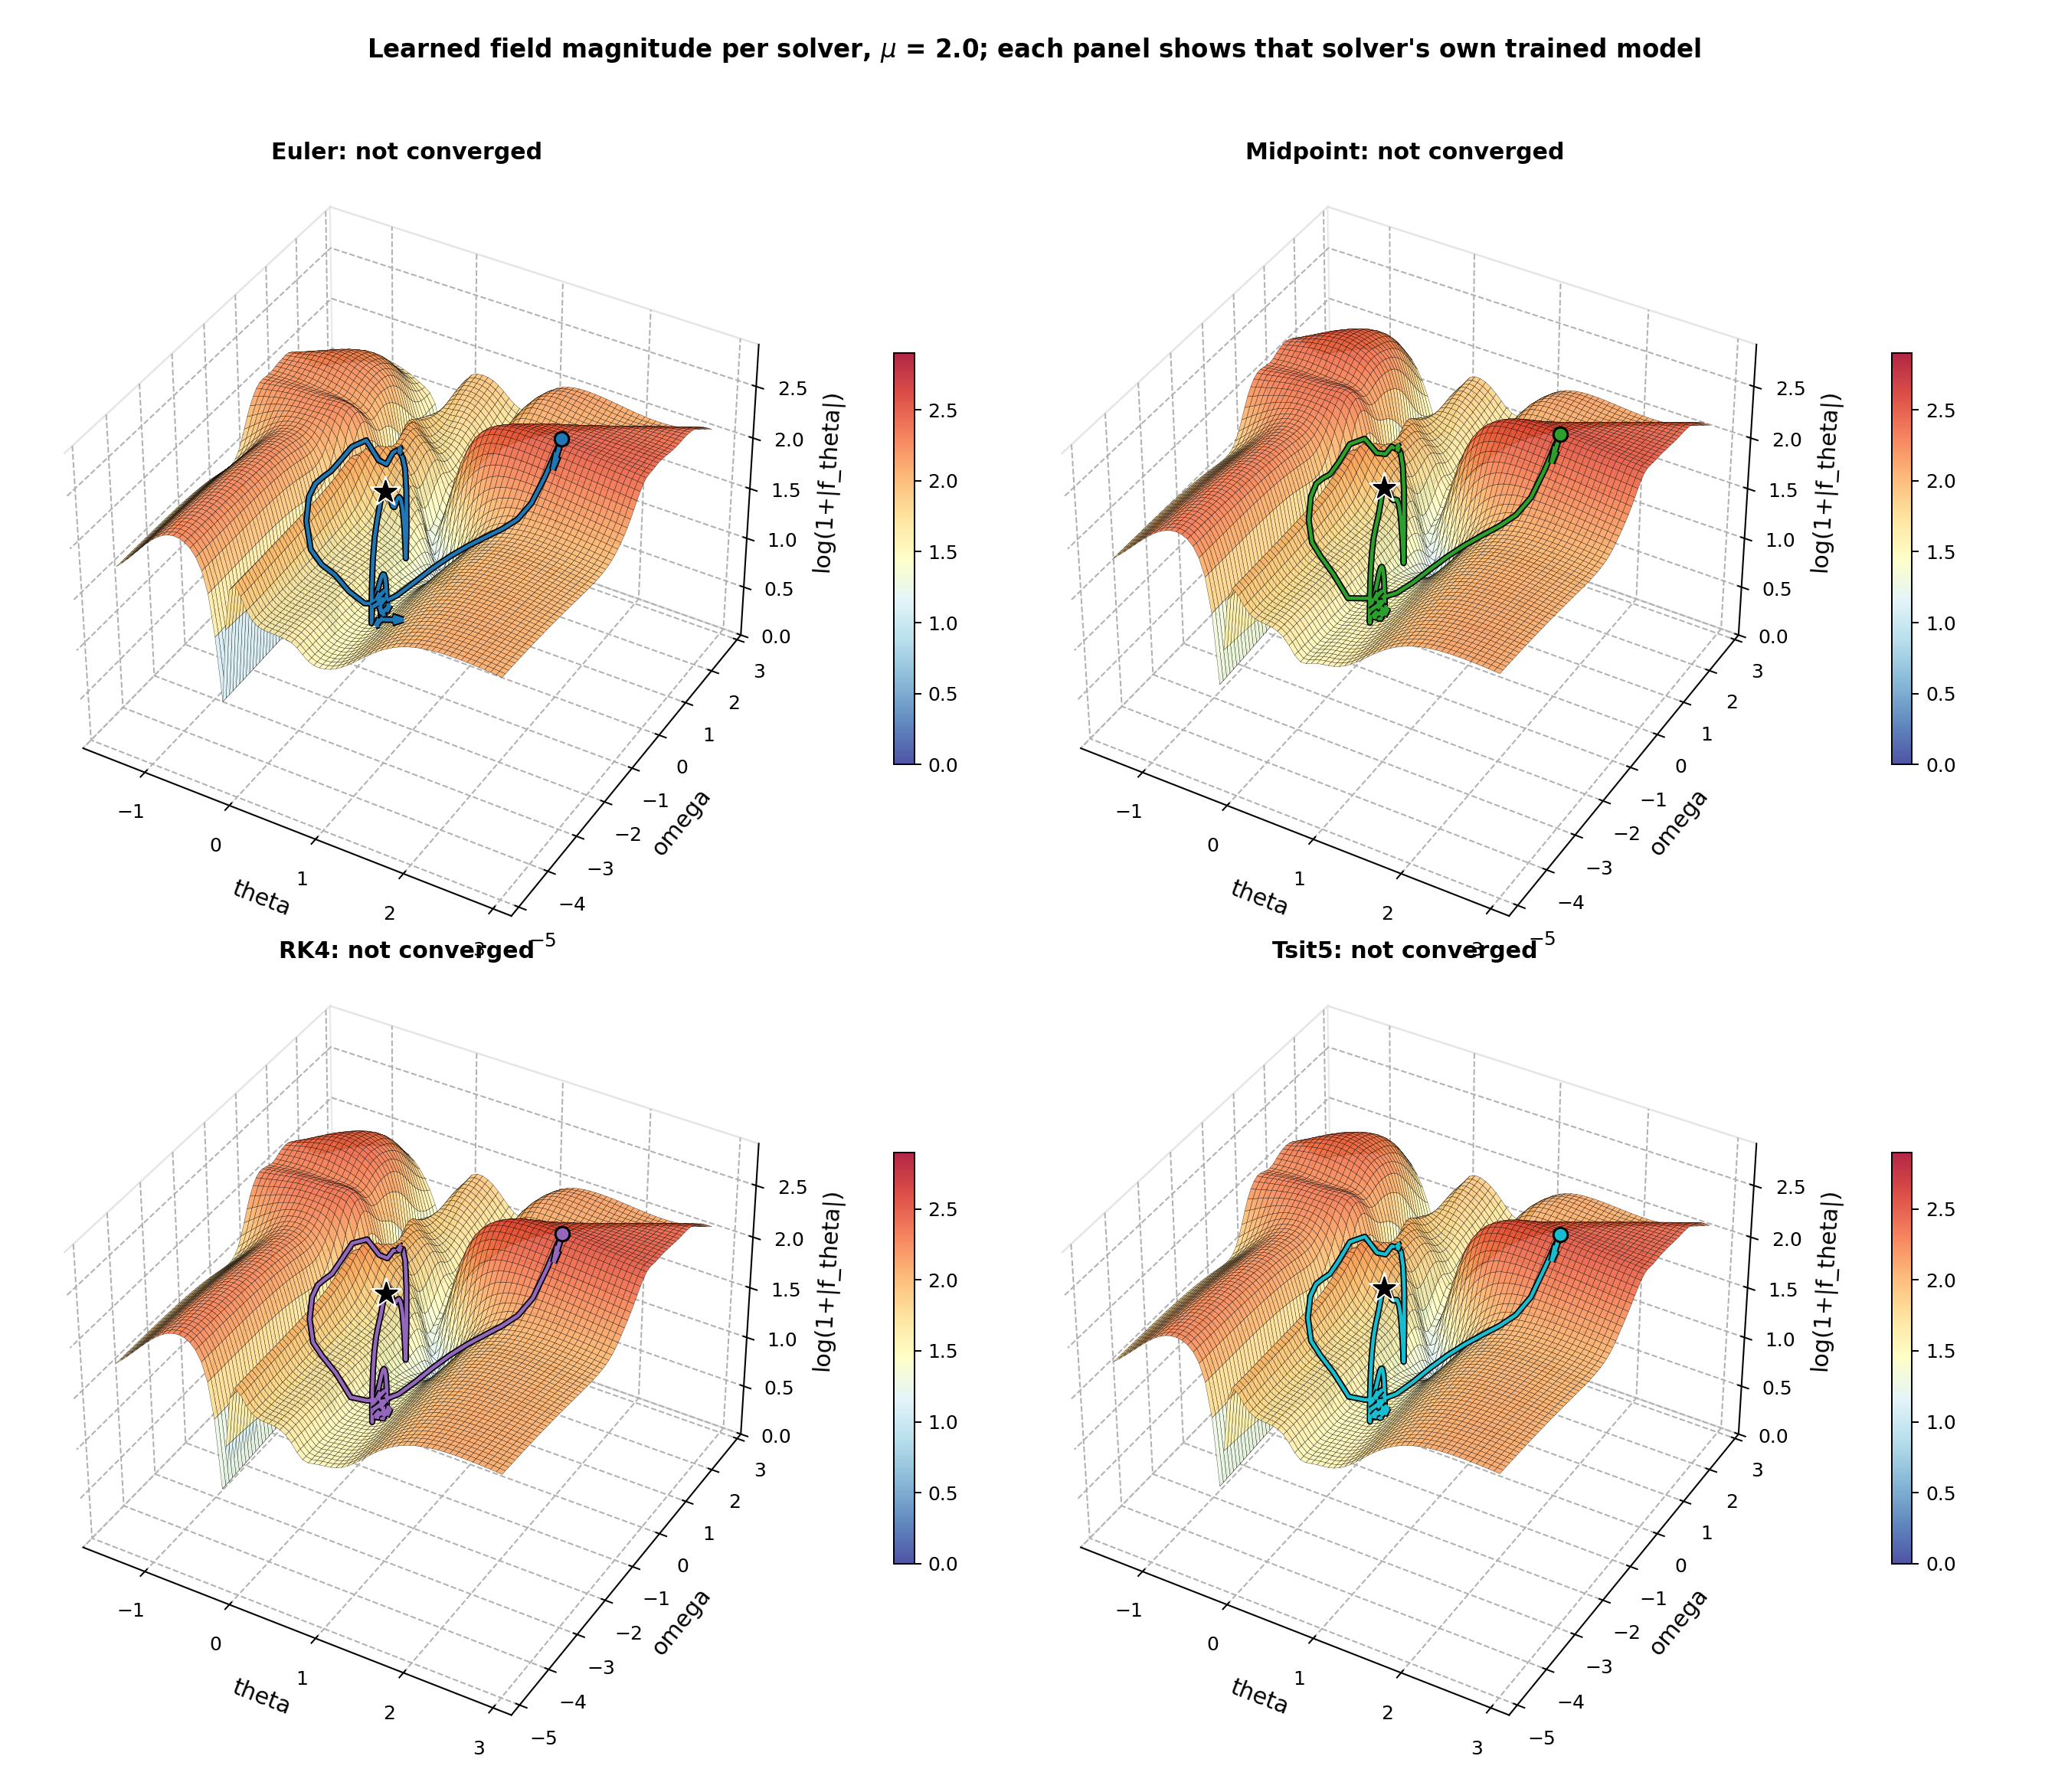
\includegraphics[width=\linewidth]{figures/track_d/phase_portrait_3d_mu2.0.png}
\end{minipage}\hfill
\begin{minipage}[t]{0.48\textwidth}
\centering
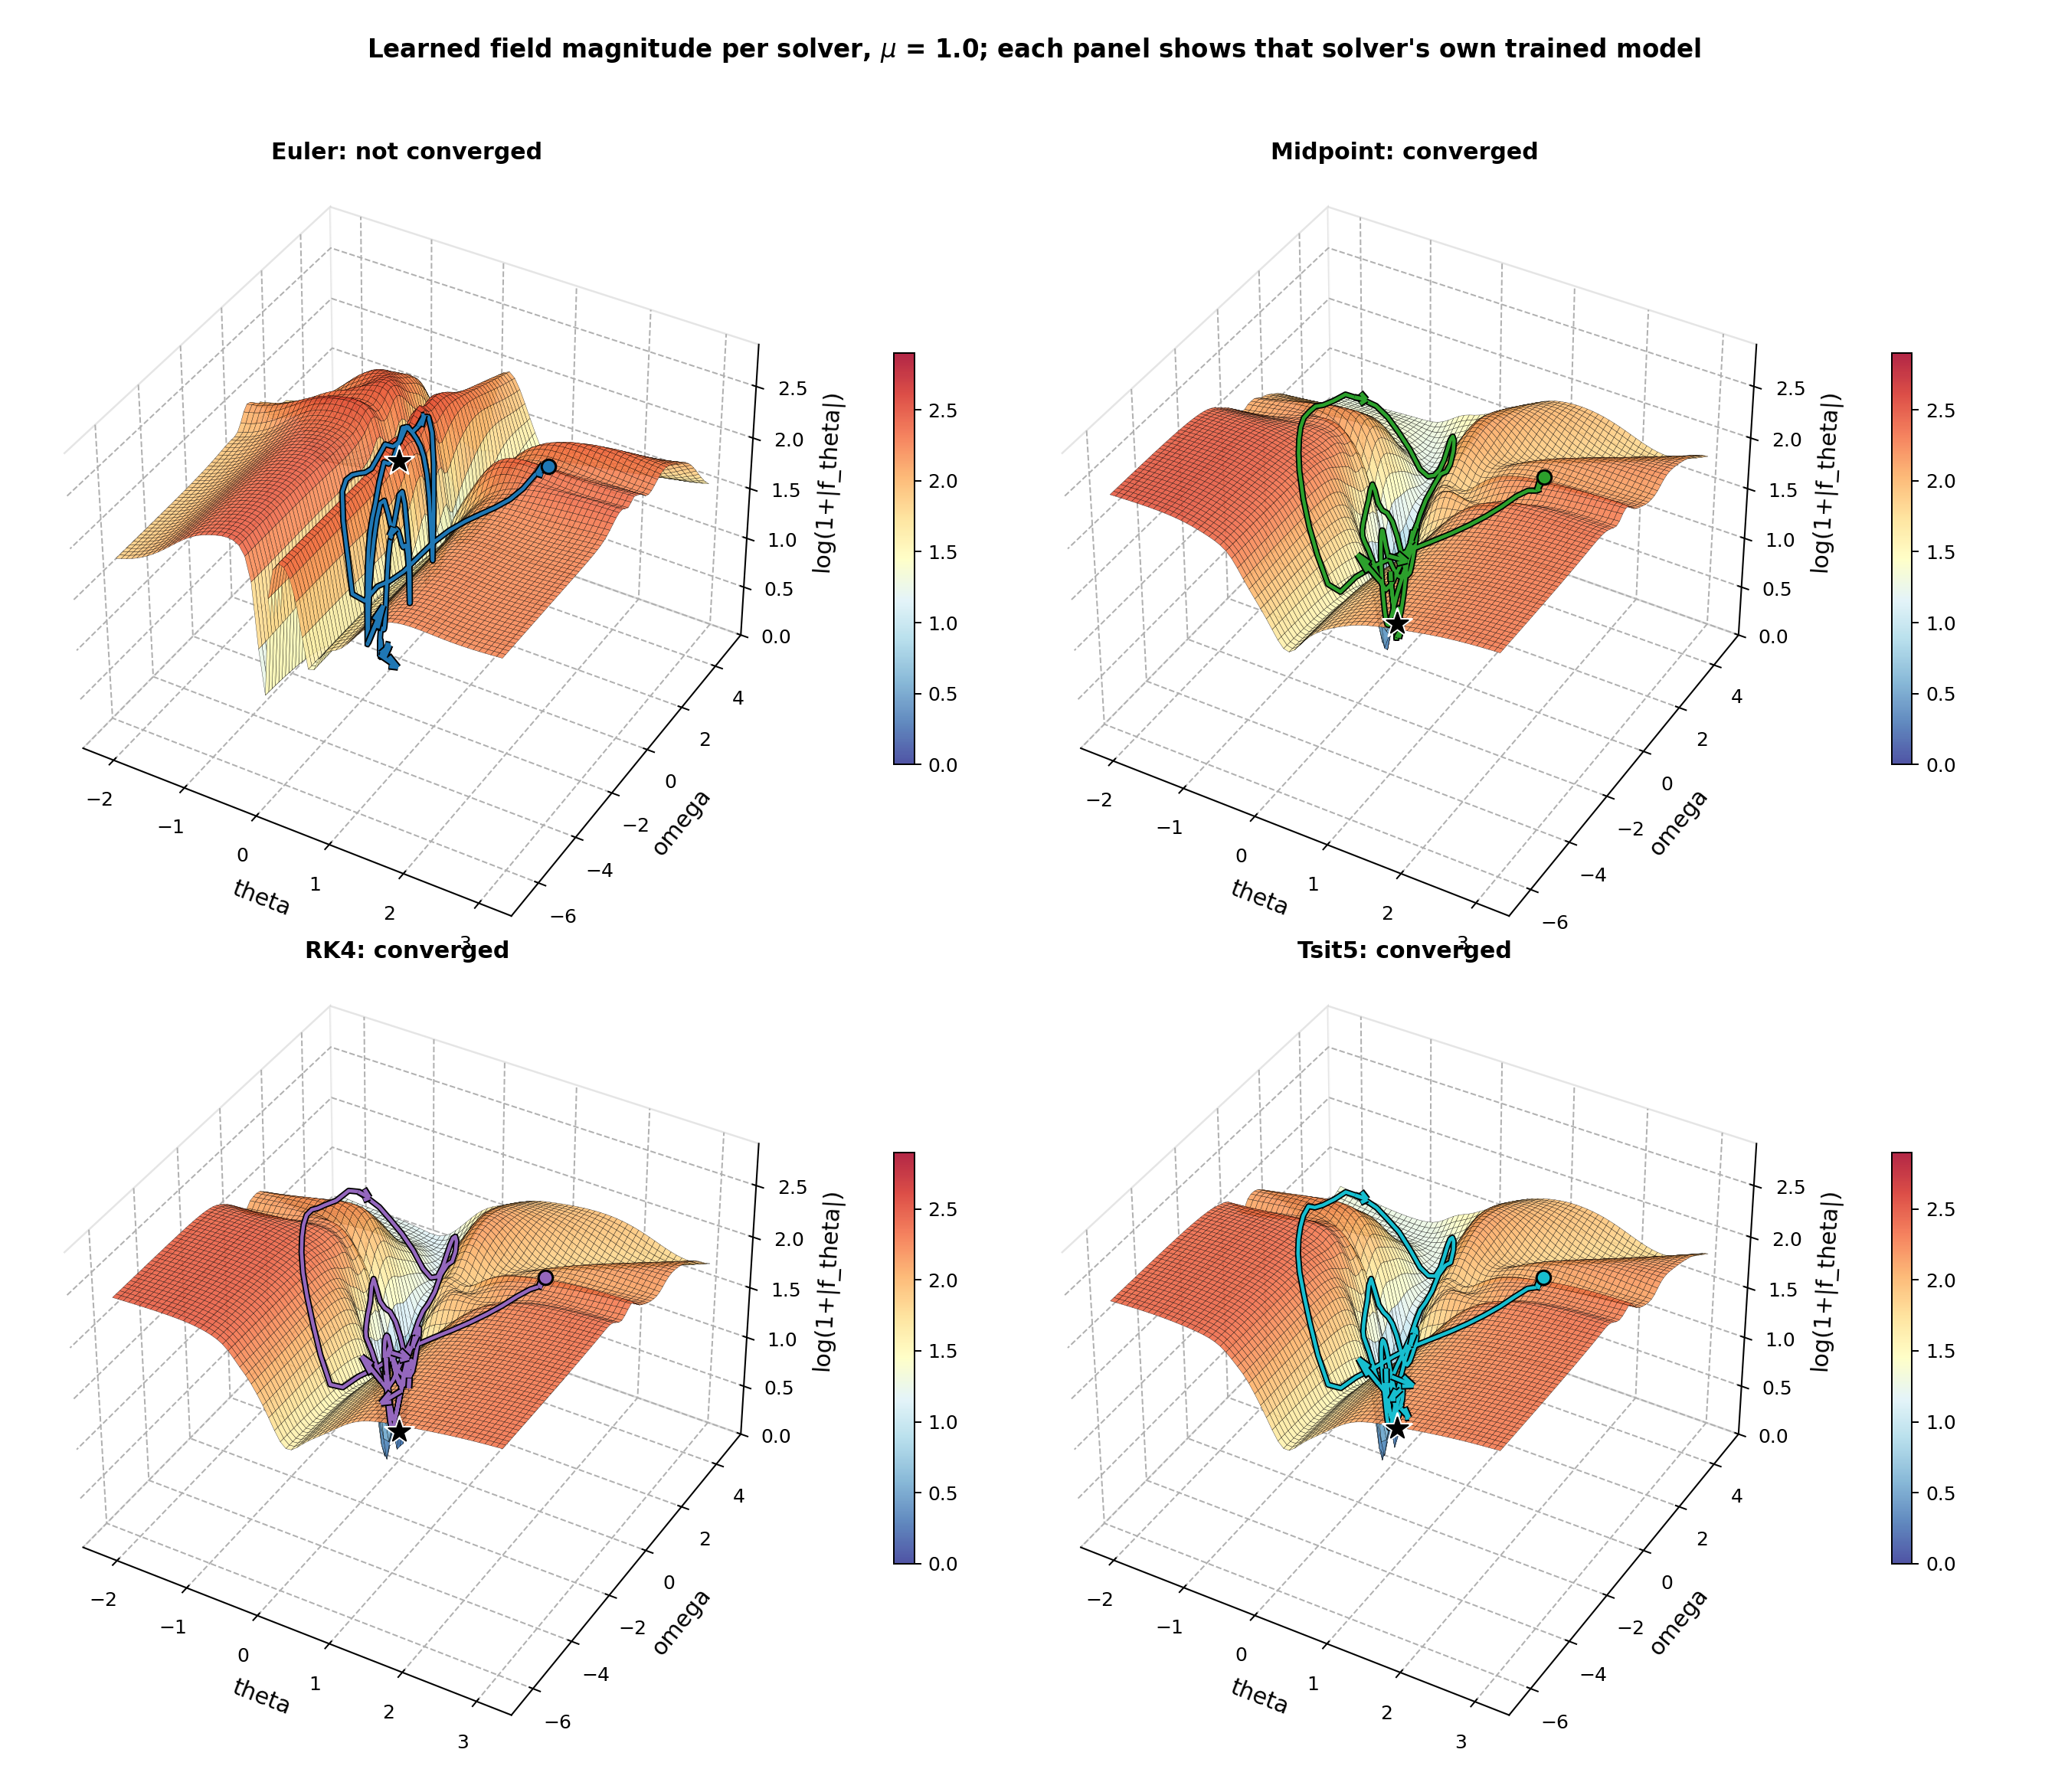
\includegraphics[width=\linewidth]{figures/track_d/phase_portrait_3d_mu1.0.png}
\end{minipage}
\caption{Learned vector-field landscape $|f_\theta(\theta,\omega)|$, per solver's
own trained model. Left ($\mu=2.0$): every solver's true equilibrium (star)
sits partway up a slope, while a separate, lower point nearby is where each
trajectory actually settles. Right ($\mu=1.0$): Euler's star sits high on a
ridge, well apart from where its trajectory spirals down and rests; for the
other three solvers, star and resting point coincide at the valley floor.}
\label{fig:phase-portraits}
\end{figure}

The full predicted trajectories tell the same story over time rather than in
a single snapshot. At $\mu=2.0$ every solver's predicted angle and angular
velocity settle onto the same wrong trajectory; at $\mu=1.0$ only Euler's
predicted angle visibly departs from the true one.
Figures~\ref{fig:mu2-collage} and~\ref{fig:mu1-collage} in
Appendix~\ref{app:stiffness-figs} show both cases panel by panel.

\subsection{Weight-space loss landscape: an independent measurement}

The phase-space plots above describe the learned dynamics; a separate
question is how forgiving the \emph{training loss} is around each solution --
whether a small nudge to the weights leaves the fit essentially unchanged or
makes it collapse. This was measured with the random-direction technique of
Li et al.\ \cite{li2018losslandscape}, adapted to KAN-ODE's 360-parameter
weight space. Two random directions $\mathbf d_1,\mathbf d_2$ are drawn and
each is rescaled parameter tensor by parameter tensor to the norm of the
corresponding trained tensor; this is a per-tensor version of Li et al.'s
filter normalization, since a KAN layer has no filters. The training MSE
$\mathcal L(\theta^\star+a\,\mathbf d_1+b\,\mathbf d_2)$ is evaluated on a
$21\times21$ grid of $(a,b)\in[-1,1]^2$, and each cell is summarized by its
\emph{rise},
\begin{equation}
\text{rise}=\log_{10}\max_{(a,b)}\mathcal L(\theta^\star+a\,\mathbf d_1+b\,\mathbf d_2)-\log_{10}\mathcal L(\theta^\star),
\label{eq:rise}
\end{equation}
the number of decades by which the loss climbs from the trained point to the
highest point of the grid.

\begin{table}[!ht]
\centering
\small
\renewcommand{\arraystretch}{1.1}
\caption{Loss-landscape rise (Equation~\ref{eq:rise}) for the seed-42
models, one random direction-pair. Bold cells are trapped.}
\label{tab:rise-seed0}
\begin{tabularx}{\textwidth}{@{}C{1.1cm} X X X X@{}}
\toprule
\hdrrow \thh{$\mu$} & \thh{euler} & \thh{midpoint} & \thh{rk4} & \thh{tsit5}\\
\midrule
1.0 & \textbf{5.53} & 9.03 & 8.99 & 9.12\\
2.0 & \textbf{4.23} & \textbf{4.24} & \textbf{4.22} & \textbf{4.20}\\
5.0 & 8.75 & 8.75 & 8.76 & 8.76\\
8.0 & 9.14 & 9.15 & 9.12 & 9.12\\
\bottomrule
\end{tabularx}
\end{table}

Read at face value, Table~\ref{tab:rise-seed0} says converged models
(rise $\approx9$) sit in steep, narrow basins, while trapped models (bold,
rise $\approx4$--$5.5$) sit on much flatter ground. That reading is
confounded. Rise is measured from the trained point, and trapped models start
from a training loss $10^2$--$10^3$ times higher than converged ones
(Table~\ref{tab:stiffness-single-seed}), so they have less room to rise even
if their surroundings are just as steep. Adding the trained-point loss back
gives the absolute height of the grid's highest point,
$\log_{10}\max\mathcal L=\text{rise}+\log_{10}\mathcal L(\theta^\star)$
(Table~\ref{tab:rise-absolute}; the trained-point loss is taken as the
recorded best training MSE, since the grids themselves were not kept).

\begin{table}[!ht]
\centering
\small
\renewcommand{\arraystretch}{1.1}
\caption{Absolute height of the loss grid, $\log_{10}\max\mathcal L$,
recovered from Table~\ref{tab:rise-seed0} and the trained-point losses of
Table~\ref{tab:stiffness-single-seed}. Bold cells are trapped.}
\label{tab:rise-absolute}
\begin{tabularx}{\textwidth}{@{}C{1.1cm} X X X X@{}}
\toprule
\hdrrow \thh{$\mu$} & \thh{Euler} & \thh{Midpoint} & \thh{RK4} & \thh{Tsit5}\\
\midrule
1.0 & \textbf{4.5} & 5.8 & 5.7 & 5.7\\
2.0 & \textbf{2.5} & \textbf{2.5} & \textbf{2.5} & \textbf{2.5}\\
5.0 & 4.5 & 4.6 & 4.6 & 4.6\\
8.0 & 4.5 & 4.5 & 4.5 & 4.5\\
\bottomrule
\end{tabularx}
\end{table}

Two different pictures emerge. For Euler at $\mu=1.0$, most of the low rise is
the starting-point effect: its rise is 3.5 decades below the converged
solvers at the same $\mu$, but its grid maximum is only 1.2 decades lower, and
it is as high as those of the converged cells at $\mu=5$ and $8$. For the
$\mu=2.0$ trap, the walls really are lower: every trapped model's grid
maximum ($10^{2.5}$) is two to three decades below every converged cell's.
Comparisons across different $\mu$ remain loose, because each $\mu$ is a
different dataset with its own loss scale. The measurement is also coarse: it
reports only the highest point of a $[-1,1]^2$ grid, not the curvature at the
minimum, which a Hessian-eigenvalue measurement would give; that was not
computed.

Figure~\ref{fig:landscape-mu2-euler} renders the $\mu=2.0$ case as a
surface: the terrain around Euler's trapped solution is broad and gently
rolling, in visual contrast to Figure~\ref{fig:landscape-mu1-tsit5}'s
converged $\mu=1.0$ solution, which sits in a narrow, sharply walled valley.
Figure~\ref{fig:landscape-mu1-euler} shows Euler's trapped $\mu=1.0$
solution, whose basin looks similarly shallow near the trained point even
though, as Table~\ref{tab:rise-absolute} shows, its far walls are as high as
a converged cell's.

\begin{figure}[htbp]
\centering
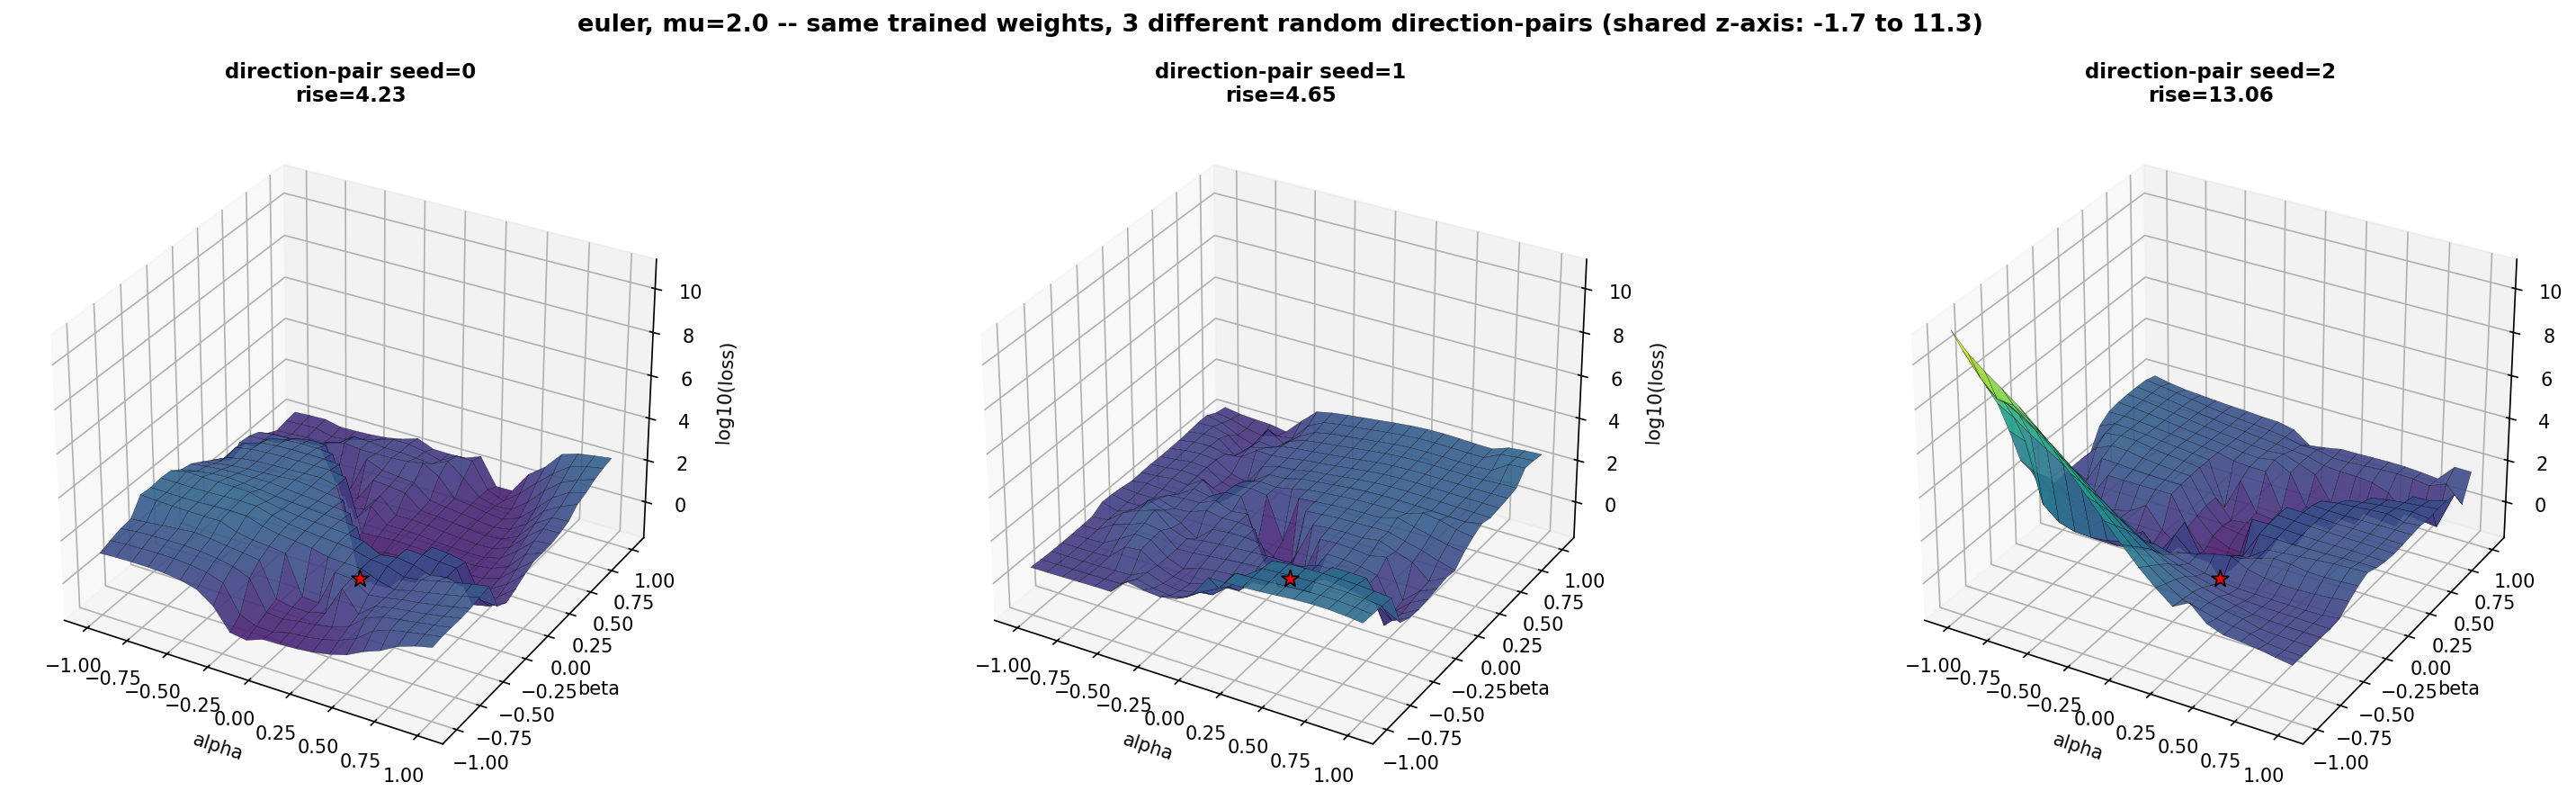
\includegraphics[width=0.95\linewidth]{figures/track_d/mu2.0_euler_direction_comparison.png}
\caption{Euler, $\mu=2.0$ (trapped): the training-loss surface around the
trained weights, viewed under three independent random direction-pairs. The
basin near the trained point (the marked star) is broad and shallow in all
three views; the third panel's steep spike on the far side is the outlier
direction discussed below, not the basin itself.}
\label{fig:landscape-mu2-euler}
\end{figure}

\begin{figure}[htbp]
\centering
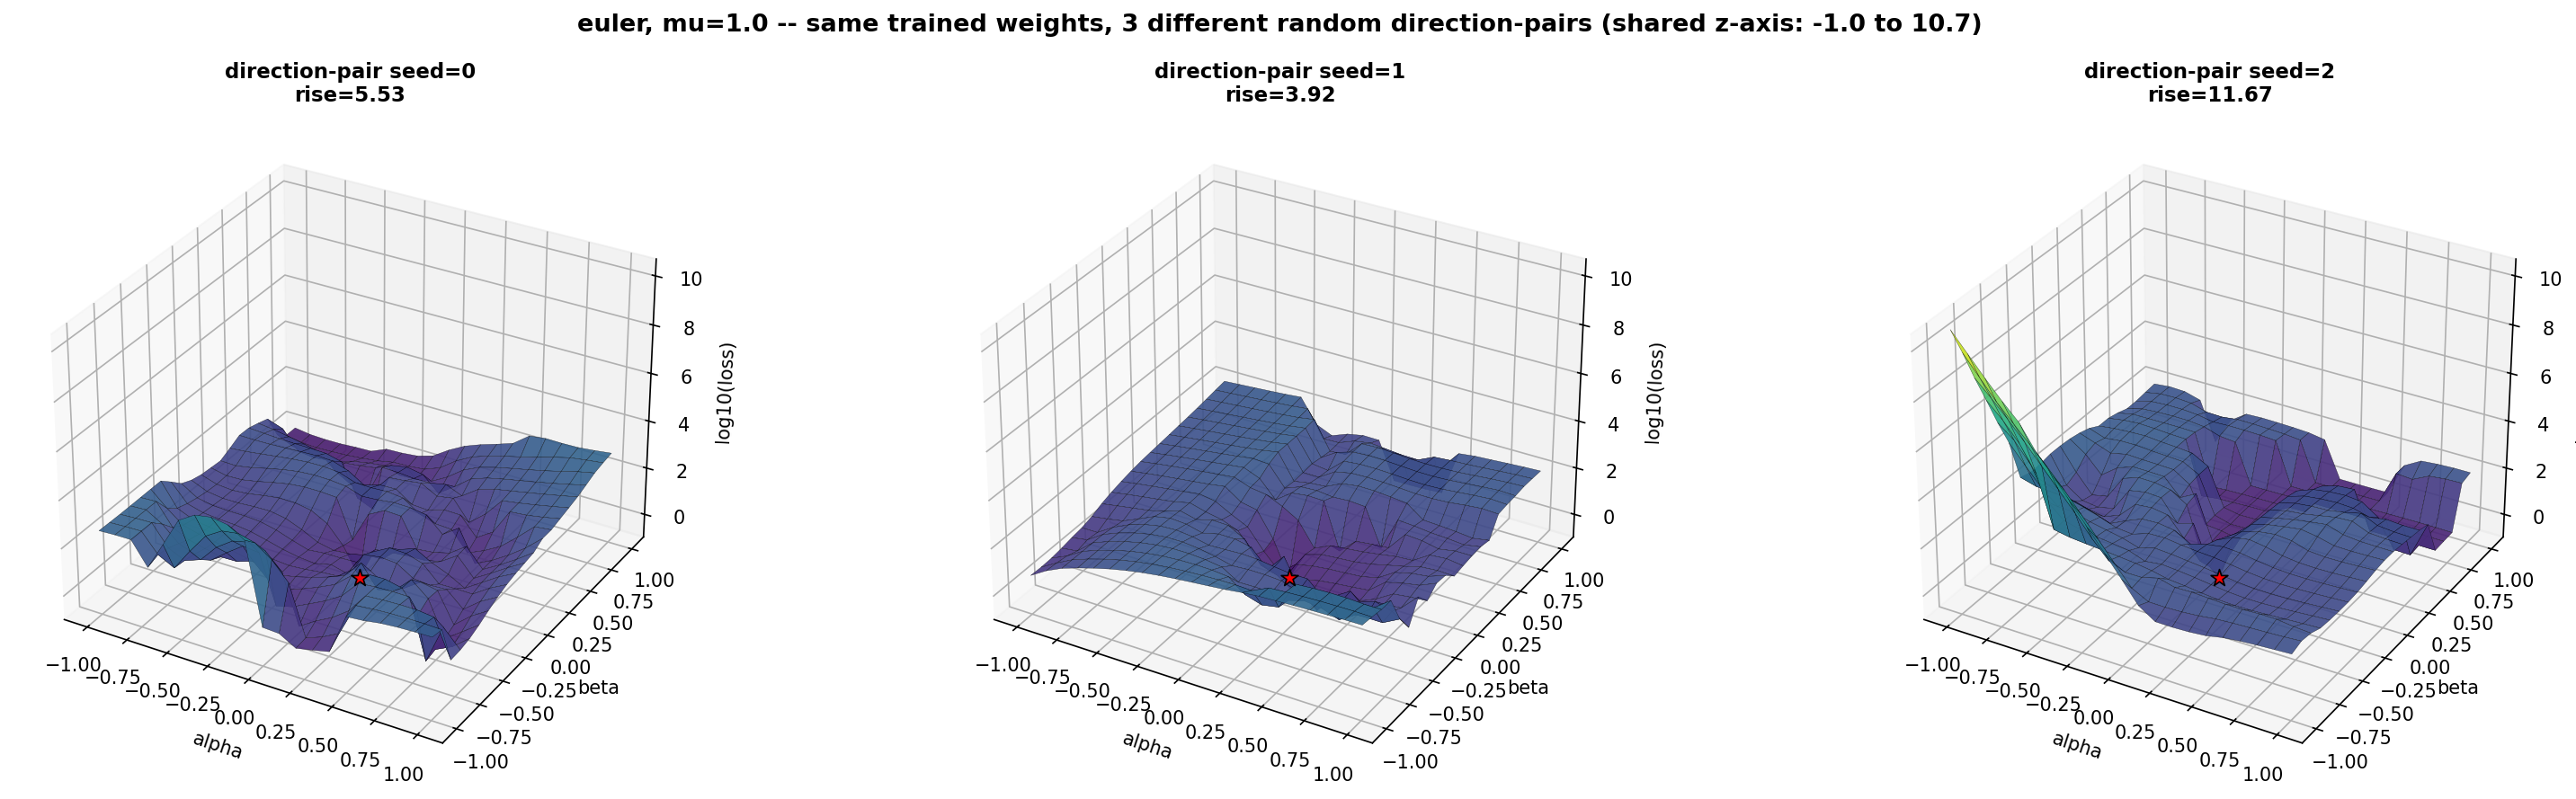
\includegraphics[width=0.95\linewidth]{figures/track_d/mu1.0_euler_direction_comparison.png}
\caption{Euler, $\mu=1.0$ (also trapped): the same broad, shallow basin shape
recurs at a different damping value under the same solver.}
\label{fig:landscape-mu1-euler}
\end{figure}

\begin{figure}[htbp]
\centering
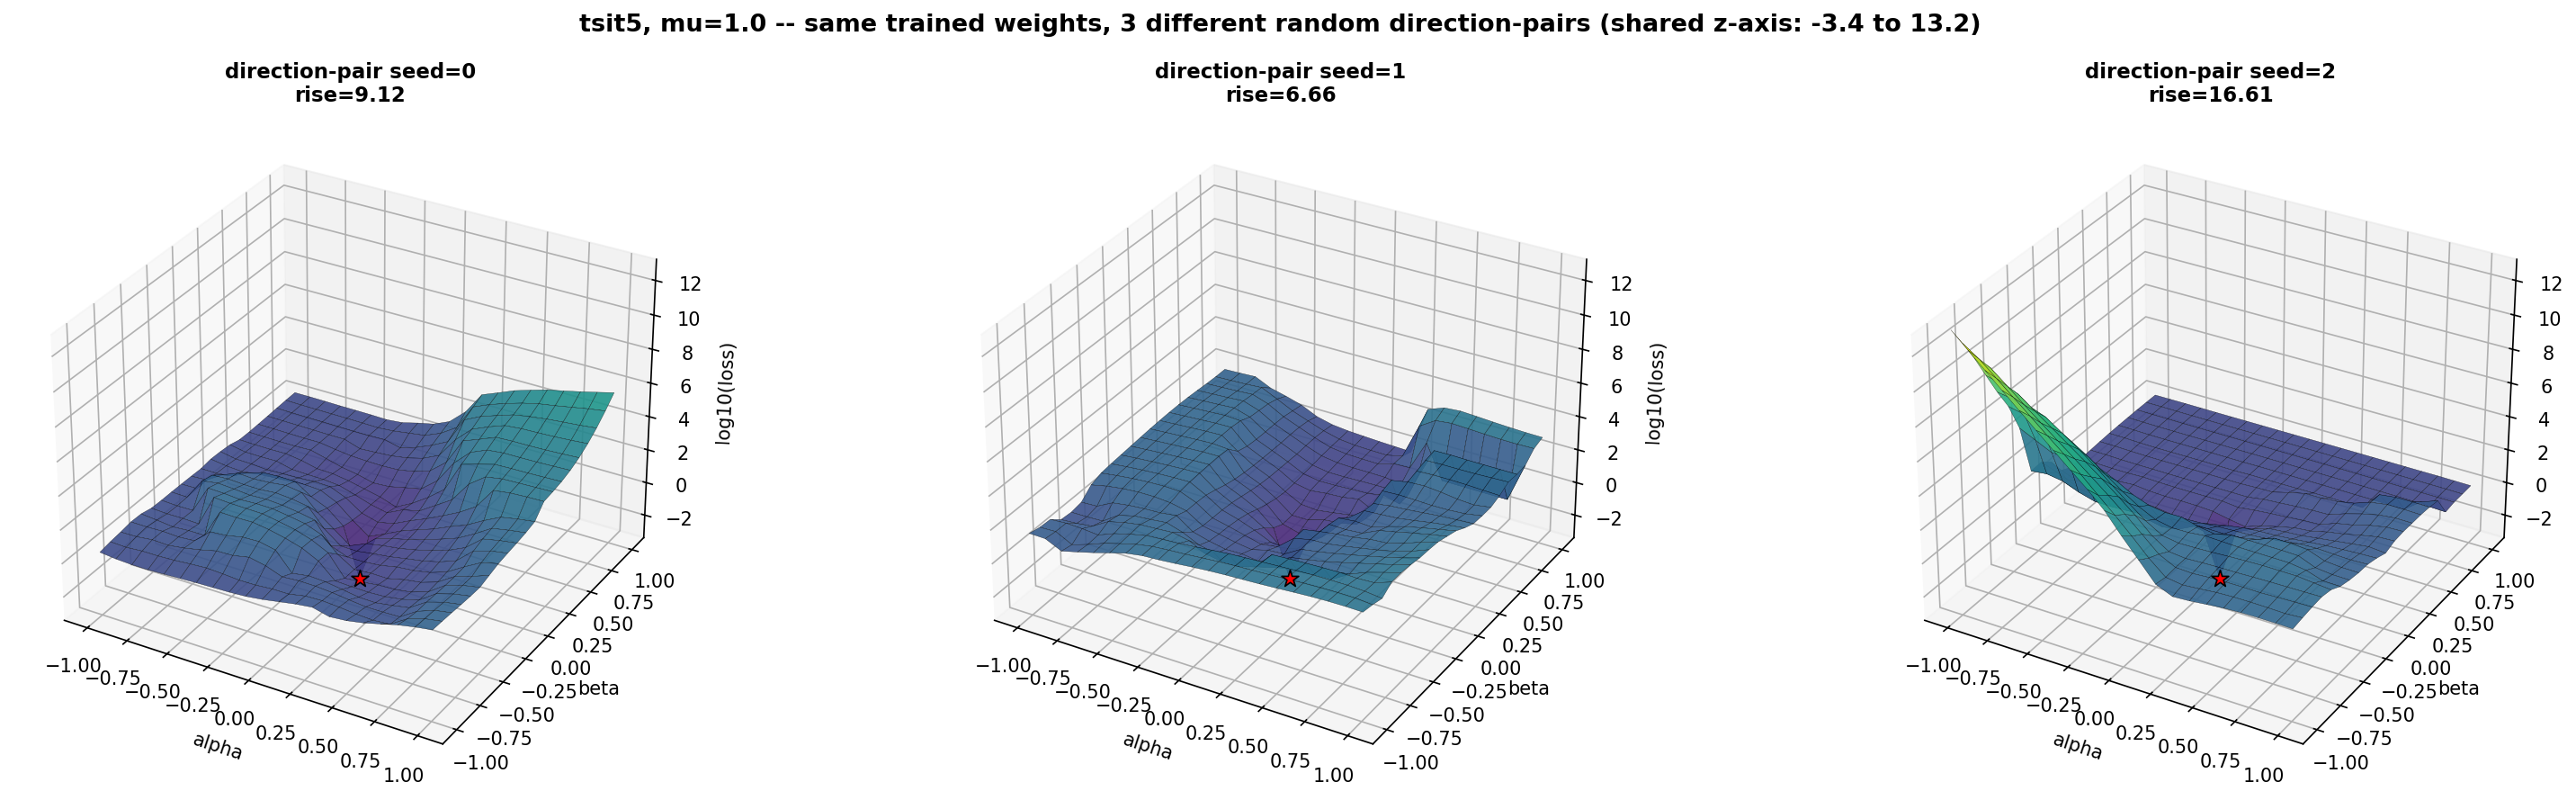
\includegraphics[width=0.95\linewidth]{figures/track_d/mu1.0_tsit5_direction_comparison.png}
\caption{Tsit5, $\mu=1.0$ (converged): the basin around the trained point is
visibly narrower and drops noticeably lower, in every one of the three
direction-pairs, than either trapped case above.}
\label{fig:landscape-mu1-tsit5}
\end{figure}

\paragraph{Robustness check across three direction-pairs.} Repeating the
measurement with two more independent random direction pairs per cell (72
measurements total) found one direction-pair acting as a shared outlier
across nearly every cell. Because every model shares the same architecture,
one particular raw random draw runs toward a steeper wall in all 24 cells at
once, inflating that direction's rise by roughly $2$--$3\times$ everywhere.
The size of the measured effect depends on how many direction choices are
averaged: the $\approx2\times$ gap between trapped and converged cells seen
with a single direction-pair narrows to roughly 25--35\% once all three
direction-pairs are
averaged, since the outlier direction inflates the trapped cells' mean more
than the converged cells' mean. The three-direction means keep the same
ordering, but their ranges across direction-pairs overlap heavily
(Figure~\ref{fig:rise-bars}), so with three directions per cell the gap is
suggestive rather than established.

\begin{figure}[htbp]
\centering
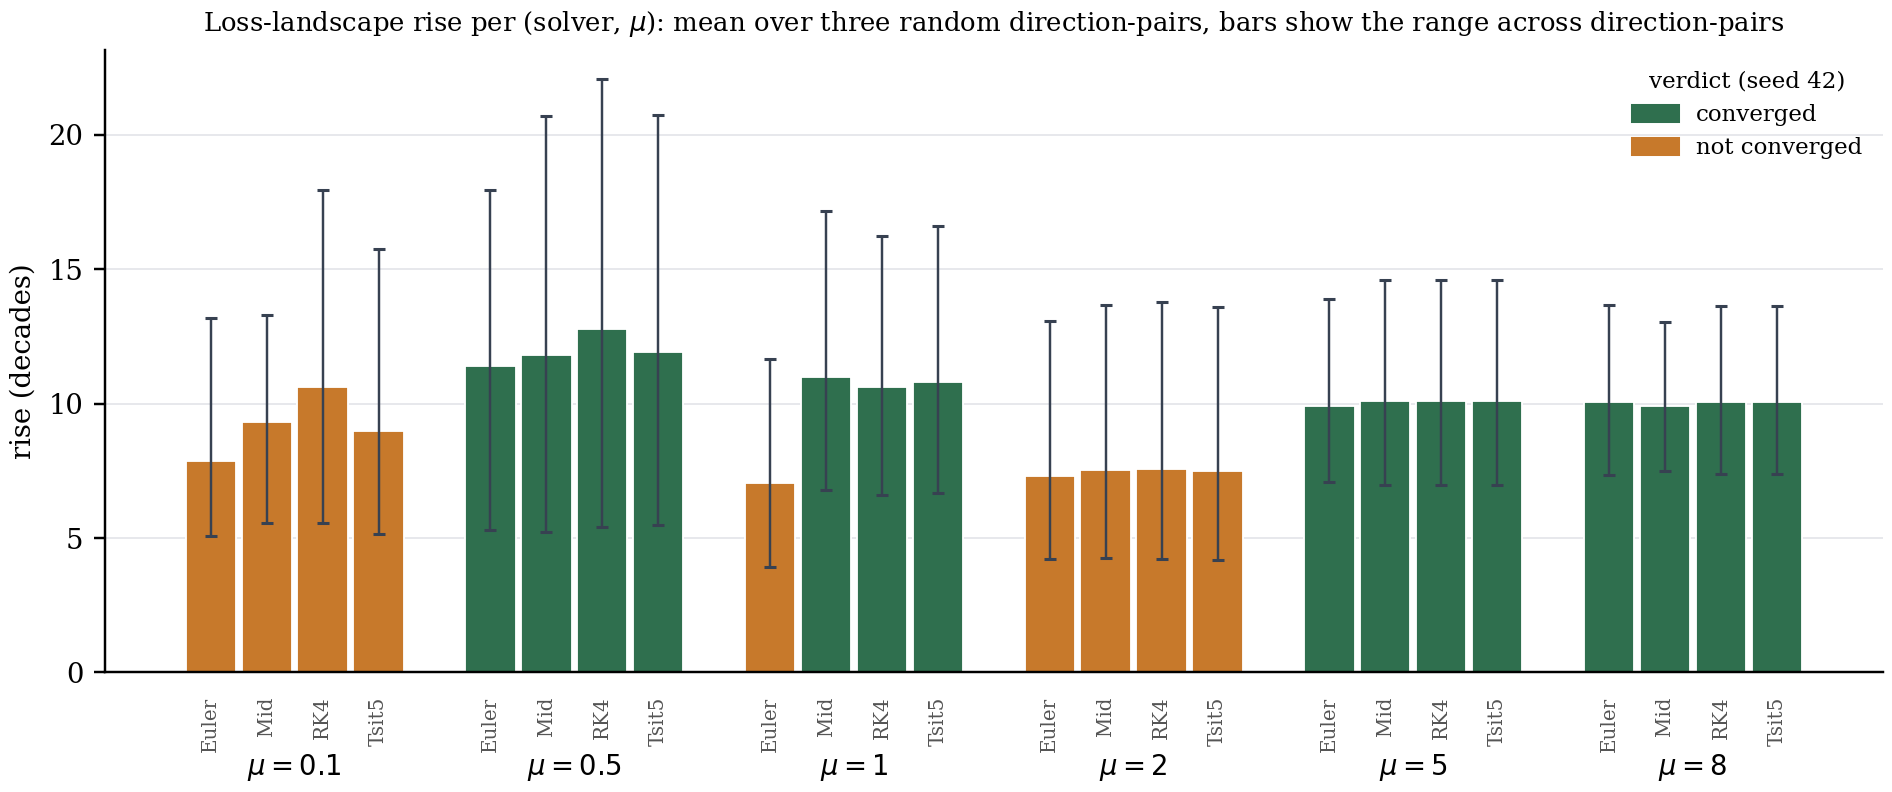
\includegraphics[width=0.85\linewidth]{figures/track_d/rise_comparison_bars.png}
\caption{Mean rise per (solver, $\mu$) over three random direction-pairs,
with the range across direction-pairs as error bars, colored by the
seed-42 verdict.}
\label{fig:rise-bars}
\end{figure}

The cells trapped by the spurious-equilibrium mechanism -- $\mu=2.0$ across
all solvers, and Euler's own $\mu=1.0$ -- sit roughly 25--35\% lower on this
chart than converged cells (mean rise $7.0$--$7.6$ against $9.9$--$12.8$; Euler
at $\mu=1.0$ is $35\%$ below the three converged solvers at the same $\mu$), a modest gap within overlapping ranges rather
than an order-of-magnitude separation, and by Table~\ref{tab:rise-absolute}
partly a starting-point effect. $\mu=0.1$ is not converged for an unrelated
reason: its trajectory never settles within the training window at all, and
its bars sit in the same range as the converged $\mu\in\{5.0,8.0\}$ cells,
occasionally above them. Whatever flatness there is belongs to the
spurious-equilibrium trap, not to every cell the classifier marks as not
converged. Figure~\ref{fig:seed-converged-fraction} summarizes all 72
seeded cells.

\begin{figure}[htbp]
\centering
\begin{minipage}[t]{0.48\textwidth}
\centering
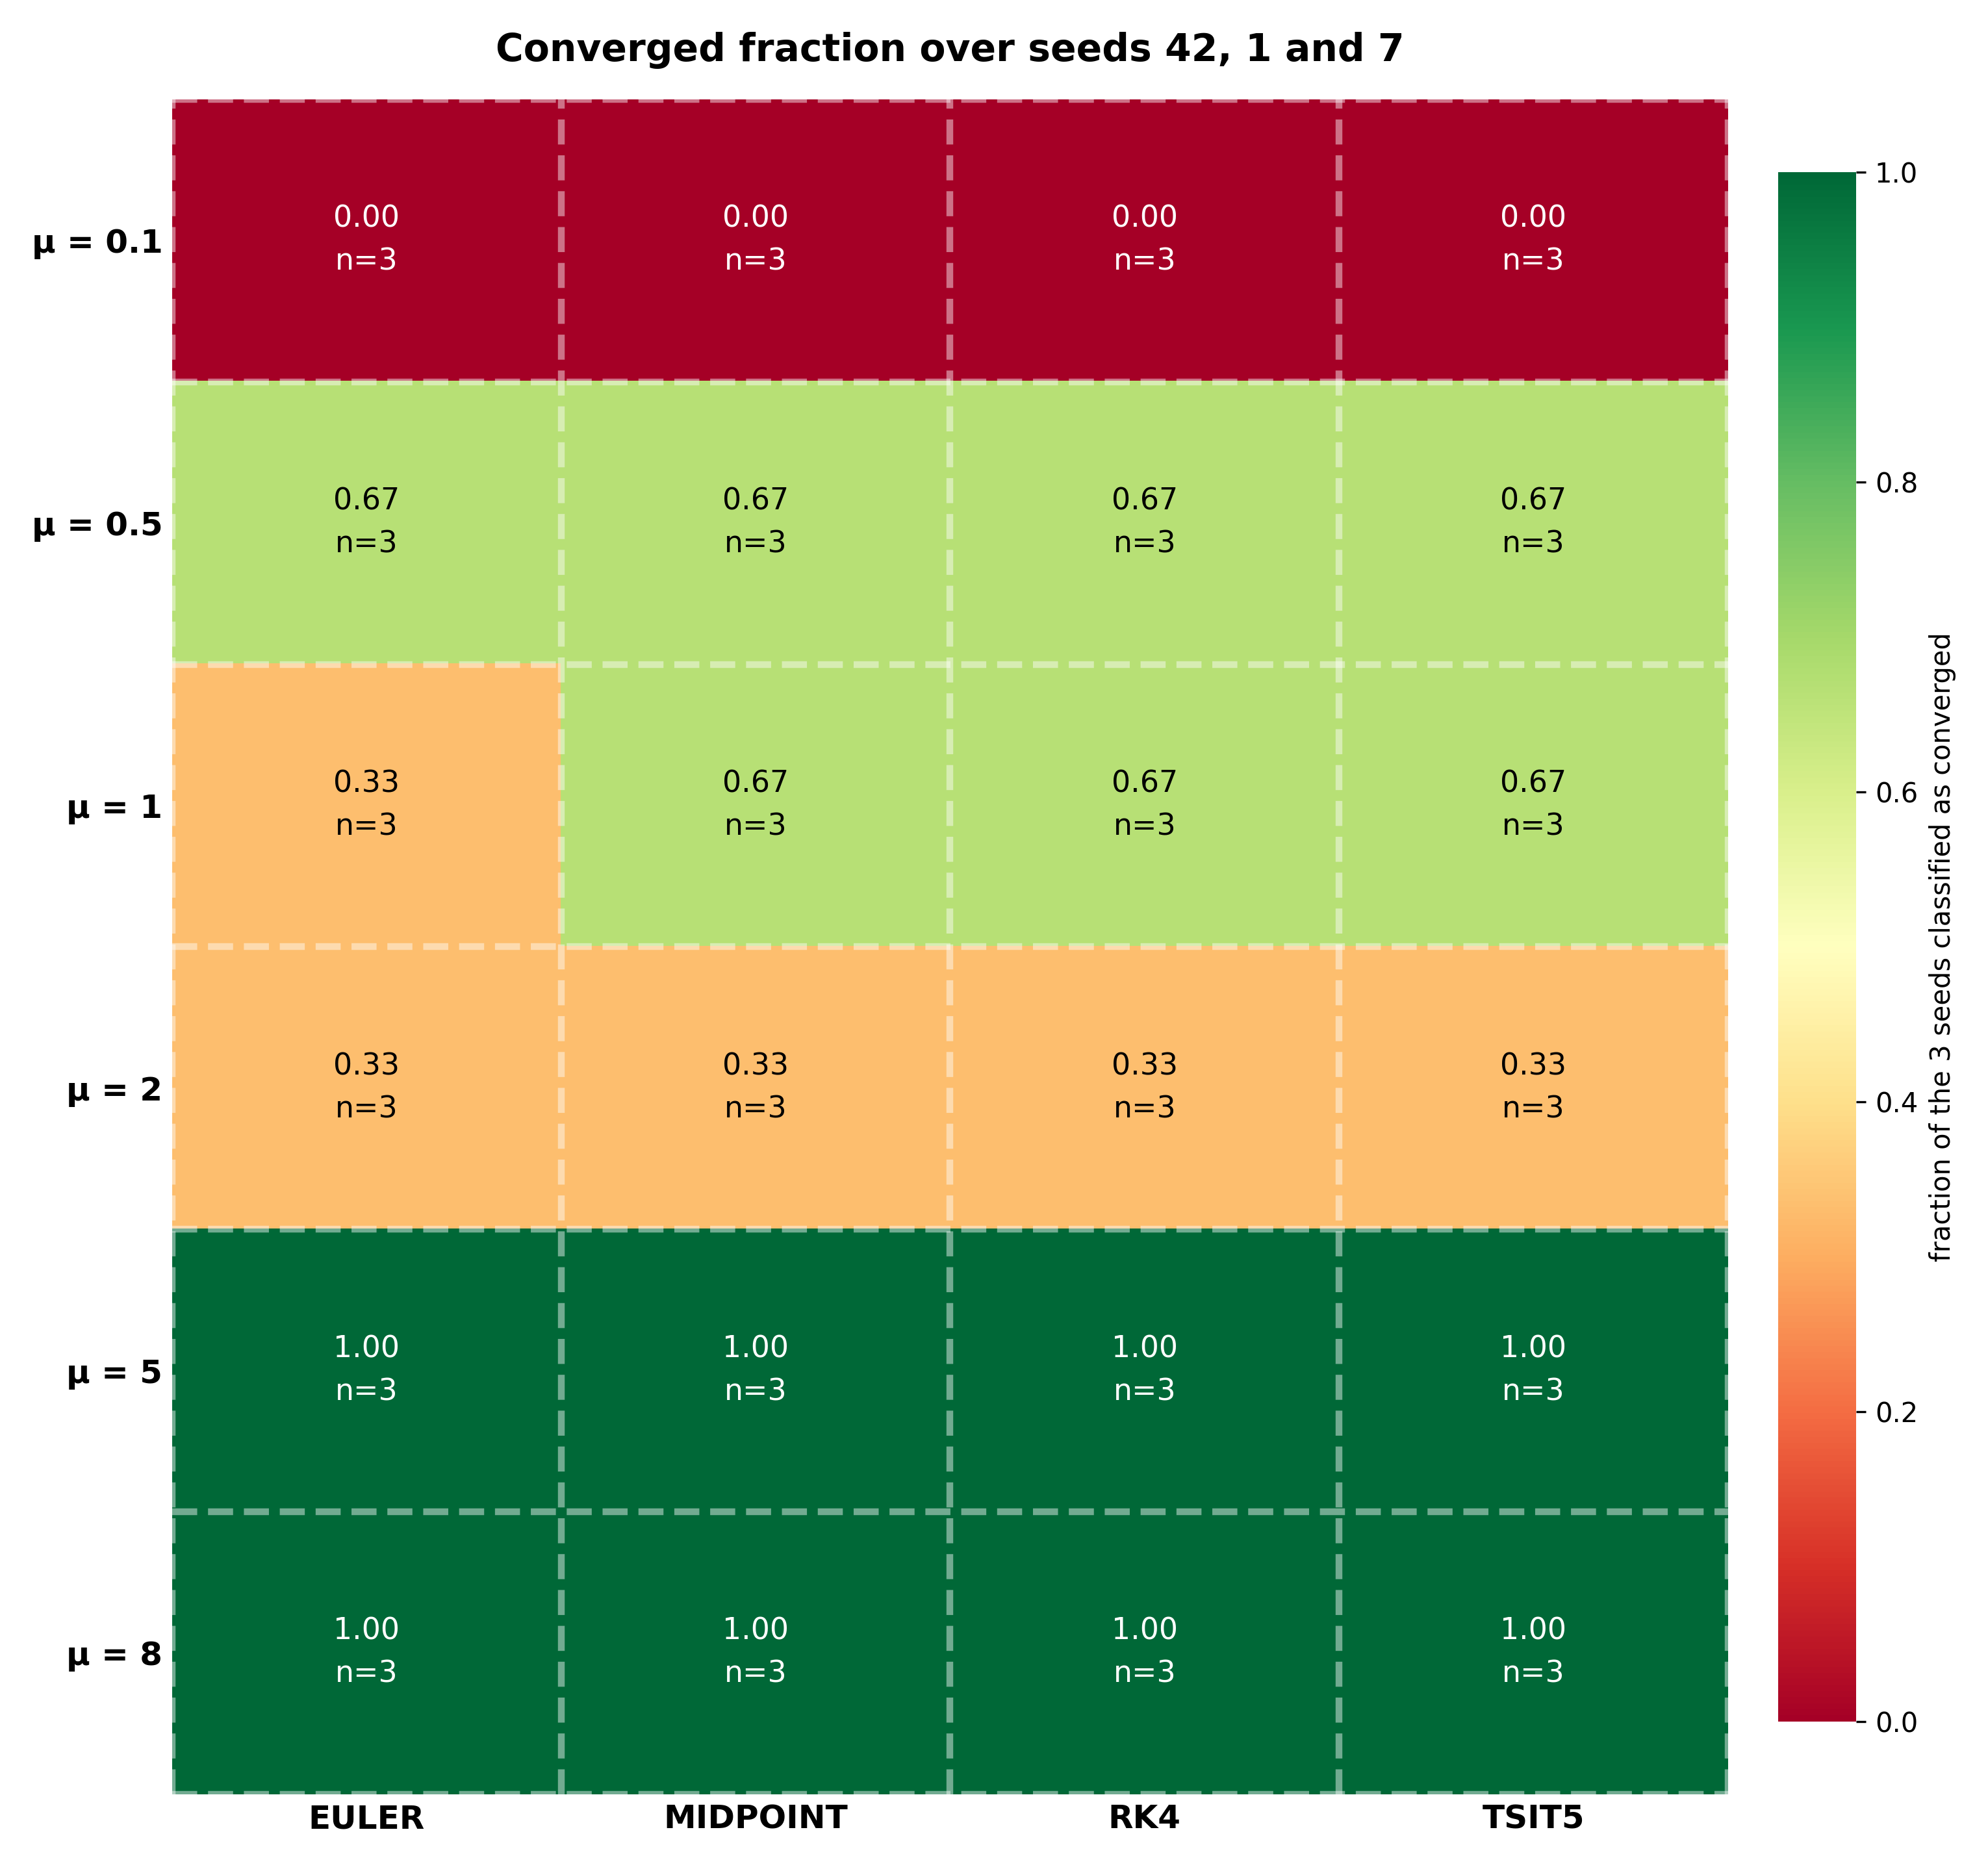
\includegraphics[width=\linewidth]{figures/track_d/seed_converged_fraction_heatmap.png}
\end{minipage}\hfill
\begin{minipage}[t]{0.48\textwidth}
\centering
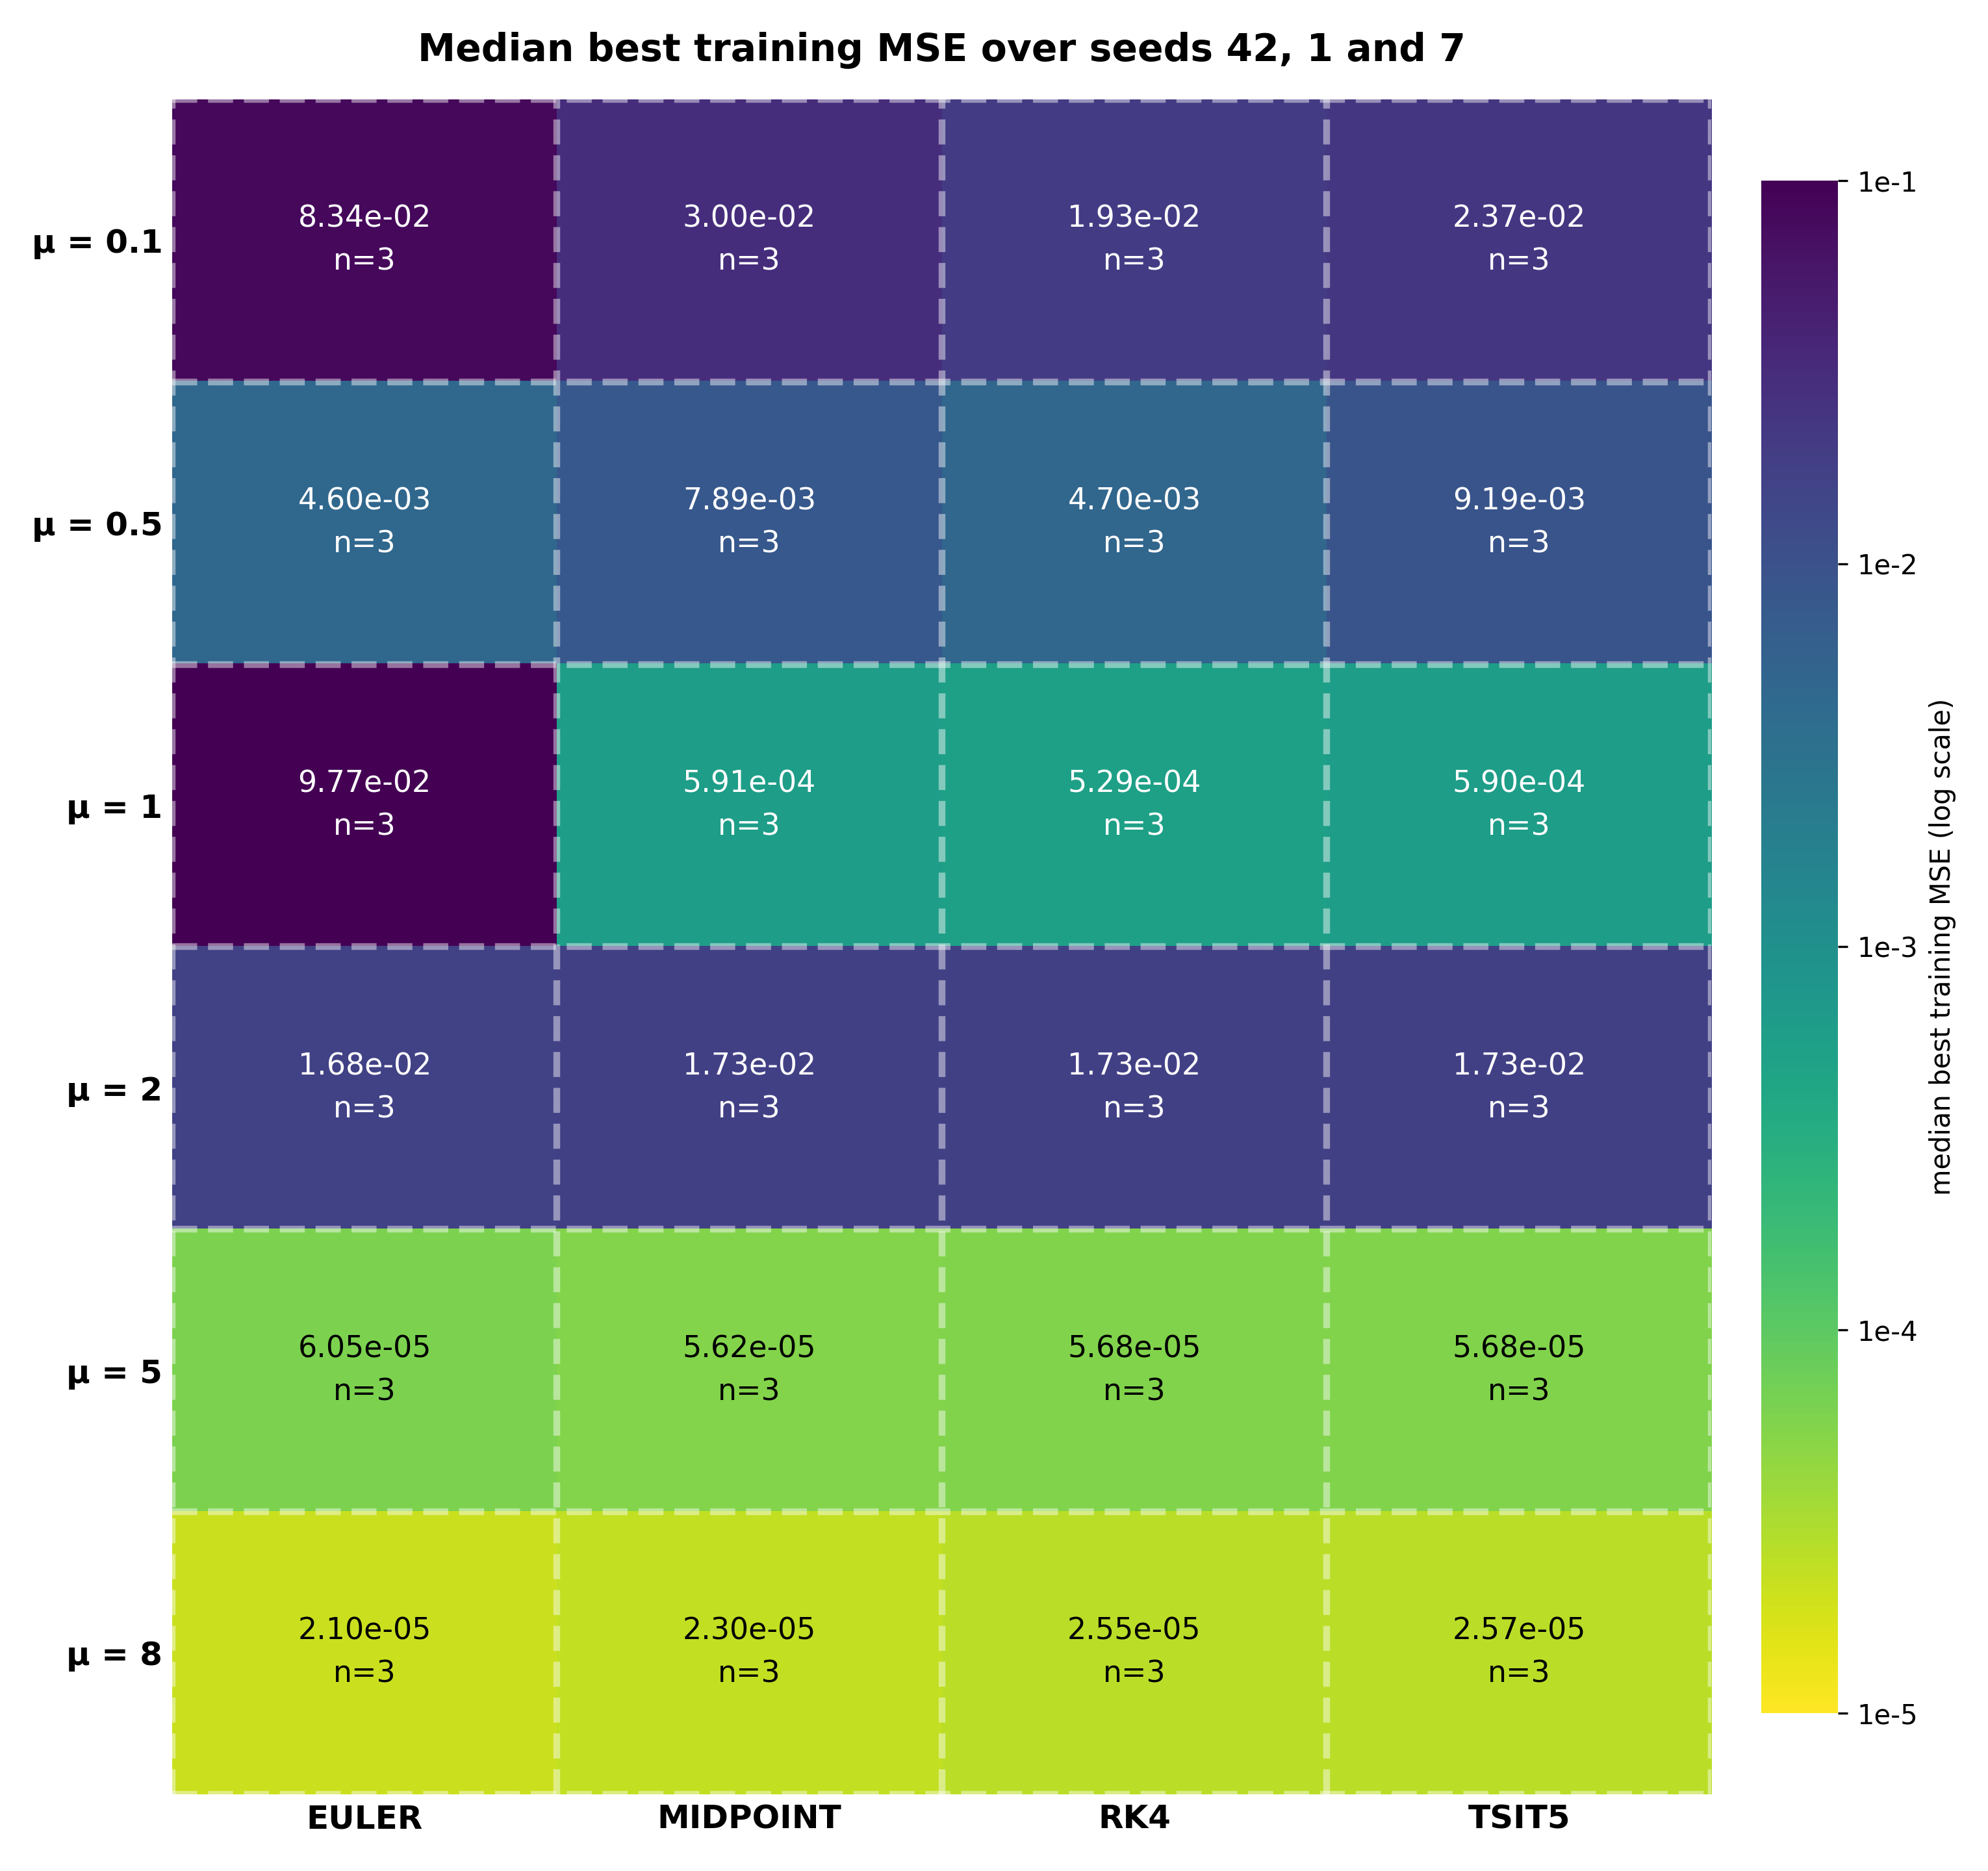
\includegraphics[width=\linewidth]{figures/track_d/seed_median_mse_heatmap.png}
\end{minipage}
\caption{Converged fraction (left) and median training MSE (right) over 3
seeds, all 4 solvers $\times$ 6 $\mu$ (72 cells). The two agree everywhere:
low converged-fraction cells are exactly the cells with elevated median
error.}
\label{fig:seed-converged-fraction}
\end{figure}

\begin{keypoint}[Verdict]
Linear stability theory predicted no divergence, for the true system and
for the trained networks, and none occurred. The sweep never reached a stiff
regime, so it cannot test stiffness itself. What decides the outcome is a
seed-dependent local minimum of training: at $\mu=2.0$ it produces a
genuine, attracting spurious equilibrium of the learned field, confirmed by
Newton's method and by its Jacobian, and shared by all four solvers trained
from the same initialization. The loss-landscape measurement is consistent
with this at $\mu=2.0$, but it is coarse and partly confounded by the
trained-point loss, so it is supporting evidence rather than an independent
proof.
\end{keypoint}

\FloatBarrier
